\section{Power balance} 
\begin{figure}[h!] 
\centering 
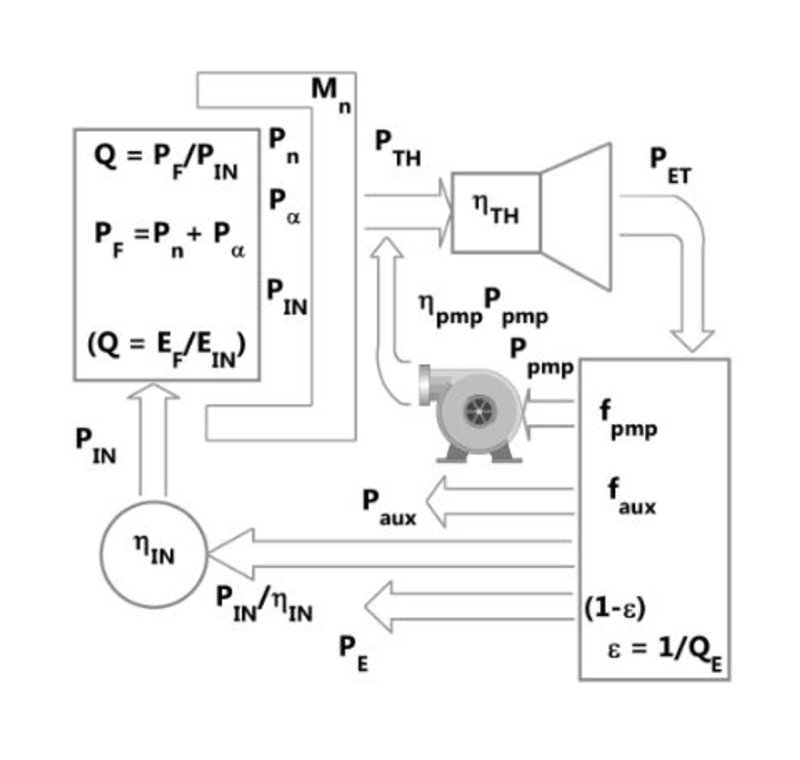
\includegraphics[scale=0.6]{StandardFigures/power.eps} 
\caption{Fusion-based electric power station power-flow diagram.}
\label{fig:pwr} 
\end{figure} 
A representative power-flow diagram for a fusion-based electric power station is presented in Fig. \ref{fig:pwr}. Power, $P_{IN}$, is input to the fusing plasma with efficiency, $\eta_{IN}$. For the D-T fuel cycle, the fusion power, $P_{F}$, is partitioned 20 \% to 3.52-MeV alpha particles and 80 \% to 14.06-MeV neutrons, is relatable to the input power by the gain, Q, as a figure of merit. In a Li-bearing blanket, the neutron power is multiplied by a factor, $M_{n} \simeq 1.1$.  The useful thermal power is $P_{TH}$, which is converted by a turbine-generator (TG) set to a gross electric power, $P_{ET}$.  A fraction of $P_{ET}$ is recirculated to provide $P_{IN}/\eta_{IN}$ as well as pumping power for the primary coolant and other housekeeping power.  The total recirculating power fraction is $\epsilon$, a figure of merit that monitors site power. The net electric power available for sale to the grid is $P_{E} = (1 - \epsilon)P_{ET}$. Not shown on the diagram is the lost power, $P_{Loss} = (1 - \eta_{TH})P_{TH} + (1 - \eta_{IN})P_{IN}/\eta_{IN}$. An alternative definition, $Q_{E} = (1 - \epsilon)/\epsilon$, is sometimes used.  In the desirable limit of low $\epsilon$, these expressions converge asymptotically. Note that the latter form is what was used recently by Wurzel and Hsu \cite{Wurzel2022}. \\

Given a stipulated target for the net electric-power output, $P_E$, the thermal-power output, $P_{TH}$, is determined for a value of the thermal conversion efficiency, $\eta_{TH}$, such that \hbox{$P_E = (1-\epsilon) \eta_{TH} P_{TH}$}, where \hbox{$\epsilon = 1/Q_E$} is the recirculating power fraction and $Q_E$ is the engineering gain.   The gross electric-power output is \hbox{$P_{ET} =\eta_{TH} P_{TH}$}. A fraction $f_{aux}$ of $P_{ET}$ ($P_{aux} = f_{aux} P_{ET}$) is allocated  for auxiliary functions (coolant and housekeeping); a fraction of the gross electric power is allocated to cryo systems, $P_{cryo}$. A fraction  $f_{pump}$ of $P_{ET}$ (\hbox{$P_{pump} = f_{pump} P_{ET}$}) is allocated for primary-loop pumping power. It is assumed that \hbox{$\eta_{pump}  \, P_{pmp}$} is recoverable as useful thermal power in the primary coolant loop.  These fractions of the gross electric power, including also the input power ($P_{IN}$) are commonly referred to as recirculating power. The engineering gain, $Q_E$, can be written as: 


\begin{eqnarray}
\label{e-2-53}
Q_E & = & \frac{1}{\epsilon} \: = \: \frac{P_{ET}}{(P_{ET} - P_{E})}  
\end{eqnarray}
\begin{eqnarray}
\label{e-2-54}
Q_{E} & = & \frac{\eta_{TH}(M_NP_{neutrons}+P_{\alpha}+P_{IN}+ \eta_{pump}P_{pump})}{(P_{aux} + P_{pump}+P_{IN}/\eta_{IN} + P_{cryo} +P_{sub} + P_{control})} 
 \end{eqnarray}
Pending detailed evaluation, the pump efficiency is taken to be $\eta_{pump} = 0.98$, the primary-coolant pumping power is $P_{pump} = f_{pump} \, P_{ET}$, and the auxiliary power is $P_{aux} = f_{aux} \, P_{ET}$, consisting of power to the coolant systems and housekeeping power.
The ratio of fusion power to input power is the fusion gain, \hbox{$Q \equiv P_{F}/P_{IN}$}, where the fusion power is $P_{F} = P_{neutrons} + P_{\alpha}$. Reworking this equation to eliminate explicit powers, the required D-T fusion gain, Q, to achieve a target recirculating power $\epsilon$ derived from the power-flow diagram to be
\begin{eqnarray}
\label{e-2-54}
Q & = & \frac{1}{(0.2 + 0.8 M_n)}
\left[\frac{(1/\eta_{TH} - f_{pump} \,\eta_{pump})(1/\eta_{IN})}{(\epsilon - f_{pump} \,\eta_{pump} - f_{aux})} - 1]\right] \: .
\end{eqnarray} 
The above equation is applicable to most steady-state D-T fusion approaches.  A design-space plot is provided as Fig. 3 of Ref. \cite{Miller2007}. For systems with some recaptured (REC: direct conversion) power, the required gain, Q, becomes: 



\begin{eqnarray} 
\label{e-2-55} 
Q & = & \left[\frac{(1/\eta_{TH} - f_{pump} , \eta_{pump})(1/\eta_{IN} - \eta_{REC})}{(\epsilon - f_{pump} , \eta_{pump} - f_{aux})} - (1 - \eta_{REC}) \right] 
\end{eqnarray}

A design-space plot with $\eta_{REC} = 0.5$ is provided as Fig. 4 of Ref. \cite{Miller2007}. \\

%For a pulsed fusion system, it is convenient to define the plasma internal energy as $W_{IN} = P_{IN}\tau_{d}$, where $tau_{d}$ is the dwell time between fusion pulses.  The fusion energy released per pulse is $W_{F}$ such that the continuous fusion power available to the primary loop is $P_{F} = W_{F}/(\tau_{d} + \tau_{b})$, where $\tau_{b}$ is the pulse (or burn) duration. Expressed in terms of energy, a gain, $Q^{*}$, can be defined as

%\begin{eqnarray} 
%Q^{*} = \frac{W_F}{W_{IN}} = \frac{P_{F}(\tau_{d} + \tau_{b})}{P_{IN}\tau_{d}} = Q(1 + \tau_b/\tau_{d})
%\end{eqnarray}

%A short $\tau_{b}$ implies a large fusion power pulse and $Q^{*}$ approaching Q.